\documentclass[12pt]{standalone}

\usepackage{tikz}
\usepackage{ctex}

\tikzset{tree/.style={every node/.style={circle, draw}}}

\begin{document}
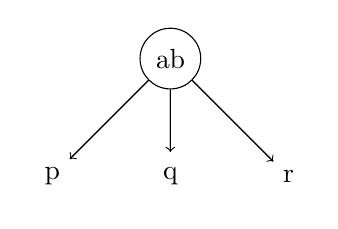
\begin{tikzpicture}

    \scoped[tree] \node at (0,0) (ab) {ab}
    child {node [draw=none] (p) {p}}
    child {node [draw=none] (q) {q}}
    child {node [draw=none] (r) {r}};

    \draw[->] (ab) -- (p);
    \draw[->] (ab) -- (q);
    \draw[->] (ab) -- (r);

\end{tikzpicture}
\end{document}
